
\section{Results}

Figure~\ref{fig:results} shows the best, average, and worst genome fitness in the population over 500 generations. Since the optimal fitness value is a minimum, and larger fitness values mean a ``worse'' genome, we negate every fitness value to obtain a more intuitive graph with the minimum at the top. Results seem fairly typical for a genetic algorithm. Average and worst fitness values are messy and have a high variance across generations. The best fitness values converge fairly quickly and do not move around much. At the end of 500 generations, the best genome had a fitness of -1326. Using the classical algorithm given this set of keys and frequencies, the actual optimal value is -1224, so this seems fairly close.

\begin{figure}[h]
    \centering
    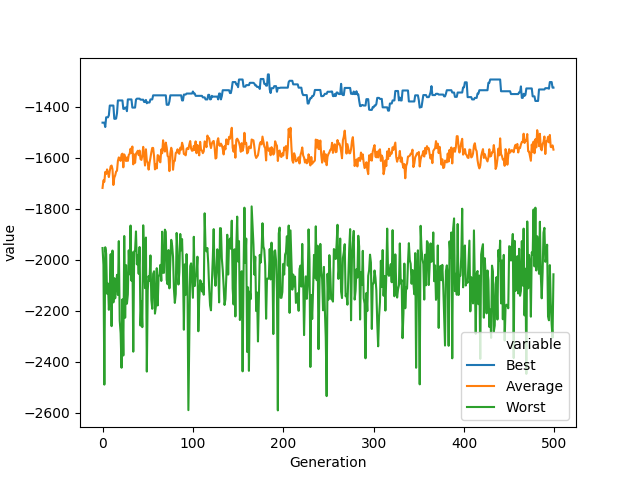
\includegraphics[scale=0.75]{figures/results.png}
    \caption{ \small Fitness results over 500 generations.}
    \label{fig:results}
\end{figure}
